\section{Arquitetura do Sistema}

    Na interseção descrita na figura \ref{fig:diagramaEstrada} existem 4 semáforos, pelo que, idealmente, cada um seria representado por uma raspberry Pi. Contudo, devido ao facto de apenas existirem duas raspberrypis disponíveis, os dois semáforos de cada sentido serão controlados por  uma das duas raspberrys e terão o mesmo comportamento. Assim, quando a raspberry Pi A está no estado VERDE é permitido o transito horizontal e quando a raspberry Pi B está VERDE é permitido o trânsito vertical. As raspberrypis nunca apresentam o mesmo estado em simultâneo. 

    O sistema foi desenhado de acordo com a figura \ref{fig:diagramaSistema}. Ambas as raspberrypis foram conectadas à rede Wi-Fi do portátil, que por sua vez comunica com o servidor NTP \url{pool.ntp.org}. Cada raspberry Pi representa um cliente que envia para o portátil os pedidos NTP de acordo com a secção \ref{sec:NTP}, que por sua vez são reencaminhados para o servidor. A resposta faz o caminho oposto. O estado da cada raspberry Pi é enviado para o portátil cada vez que existe uma transição. Este processo serve apenas para monitorização e está representado na figura como monitor. O monitor regista o tempo local da chegada da mensagem de mudança de estado de cada raspberry Pi e guarda o valor num ficheiro .txt. Por exemplo, A fica VERMELHO e B fica VERDE, o monitor mostra o tempo de cada transição (que deve ser muito semelhante).

    O protocolo empregue para a comunicação é o "Transmission Control Protocol" - TCP. Se o servidor NTP não responder à solicitação, é acionado um "timeout", e o sistema tenta restabelecer a ligação. Esta funcionalidade permite que a sincronização continue sem que o servidor esteja disponível, utilizando os último valores registados.

    \begin{figure}[h]
        \centering
        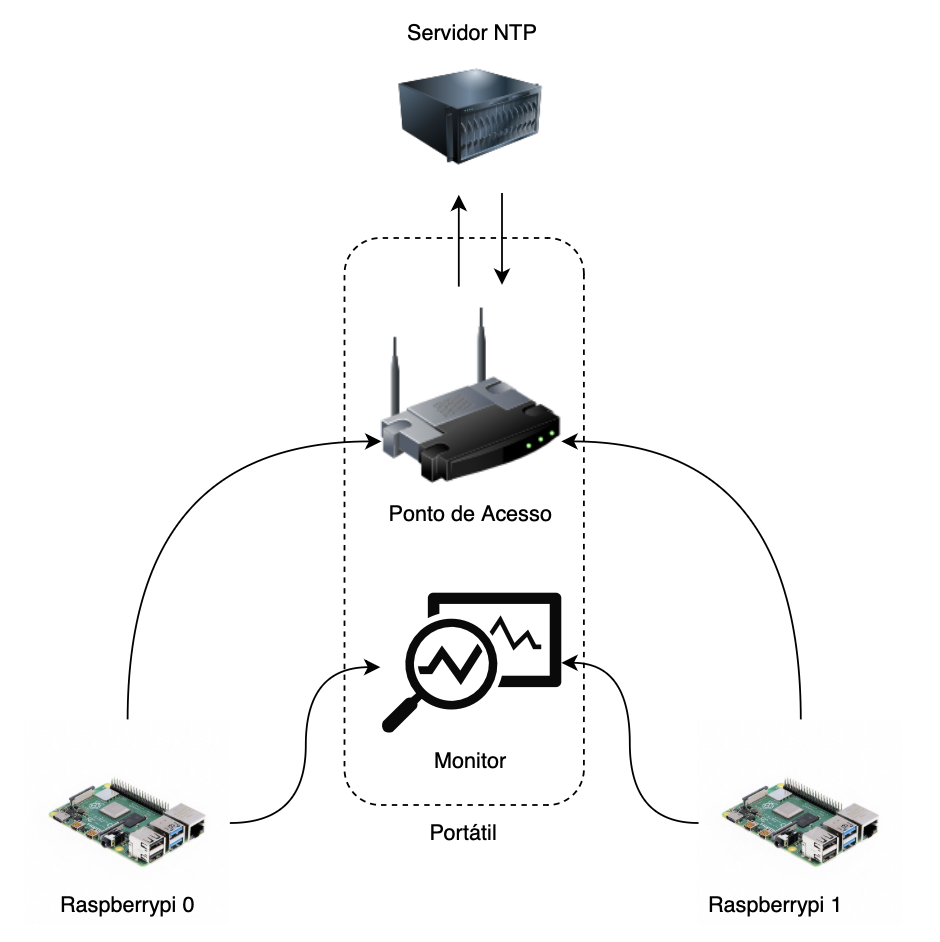
\includegraphics[width=0.8\linewidth]{figures/diagramaSistema.png}
        \caption{Diagrama da arquitetura do sistema \cite{b1}}
        \label{fig:diagramaSistema}
    \end{figure}